\pagebreak

\chapter{Jenkins}
Bei Jenkins handelt es sich um einen der bekanntesten Vertreter der Open Source CI Tools. Es hat eine sehr breite Anwenderbasis und dementsprechend sind auch viele nützliche Blog-Einträge und Hands-On-Berichte verfügbar.
\section{Geschichte}
2004 startete Kohsuke Kawaguchi damit Jenkins zu implementieren, damals noch unter dem Namen "`Hudson"' und als privates Projekt. Eigentlich wollte er nur ein Tool für sich selbst entwickeln, das ihm half, qualitativ hochwertigen Code in das SCM einzufügen. (Foreword of \cite{smart2011jenkins}).\\
Das war im Jahr 2004, und er führte das Projekt neben seiner Arbeit für SUN als privates Projekt bis 2008 weiter. Zu diesem Zeitpunkt entdeckte sein Arbeitgeber das Potential dieses Tools und er wurde gefragt, ob er nicht seine komplette Arbeitszeit für das Tool verwenden möchte, um es auf eine professionellere Ebene zu heben. Er willigte ein und bis zum Jahr 2010 erreichte Hudson einen Marktanteil von 70\%.\cite[3]{smart2011jenkins}\\
In der Zwischenzeit hatte Oracle die Firma SUN gekauft und damit auch Hudson. Ende 2010 kam es zum Zerwürfnis zwischen den Open Source begeisterten Kernentwicklern und Oracle, in welche Richtung das Projekt ausgerichtet werden sollte. Die Meinungsverschiedenheiten konnten nicht bewältigt werden, so dass im Januar 2011 die ursprünglichen Hudson Entwickler unter der Führung von Kohsuke Kawaguchi einen Fork bei GitHub erstellten unter dem Namen "`Jenkins"'. Auch die meisten der bisherigen Hudson Nutzer blieben dem Projekt treu und so wechselten 75\% der Hudson Nutzer zu Jenkins. \cite[3-4]{smart2011jenkins}
\section{Möglichkeiten des Betriebs}
Anfänglich war das Betreiben einer Jenkins Installation  eindeutig vorgegeben. Man musste gewisse Voraussetzungen erfüllen, wie z.B. Java-Installation und ein SCM-Client, und installierte dann lokal auf einem Rechner. Mittlerweile gibt es jedoch, aufgrund neuer Technologien, auch andere Ansätze, von denen ich hier drei vorstellen möchte.
\subsection{Installation direkt im Betriebssystem}
Der klassische Weg einen Jenkins CI Server zu betreiben ist die Installation direkt innerhalb eines Betriebssystems.
\begin{wrapfigure}{l}{0.5\textwidth}
  \begin{center}
    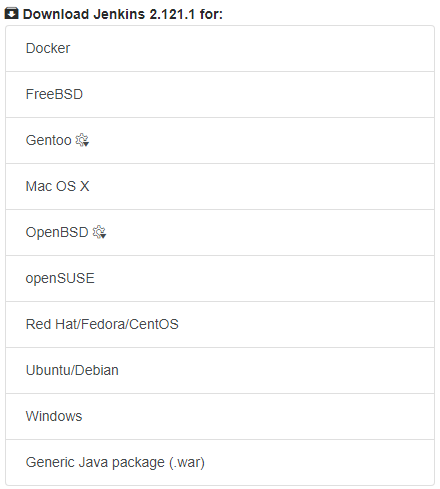
\includegraphics[width=0.48\textwidth]{./Images/Jenkins_installation_and_setup.png}
  \end{center}
  \caption{Unterstützte Installationen auf der Jenkins Seite\cite{jenkins-download}}\label{fig:Jenkins_installation_and_setup}
\end{wrapfigure}
Dazu benötigt man vor allem Java, wobei die einzige momentan unterstützte Version Java 8 ist.\cite{jenkins-java} Desweiteren werden mindestens 256MB RAM und 1GB  Massenspeicher vorausgesetzt (1GB RAM, 50GB Massenspeicher empfohlen).\cite{jenkins-installing}
\subsubsection*{Windows}
Die Jenkins Seite bietet direkt einen Windows Installer für Jenkins an. Dieser installiert Jenkins als Windows Service, der keine Interaktion des Nutzers benötigt und direkt beim Systemstart mit gestartet wird. Auch die Agenten, die die Builds ausführen, können direkt als Windows Service gestartet werden. \cite{jenkins-windows}\\
Außerdem wird die Installation von "`Unix-Utils"'\footnote{Das sind Tools, die Unix-like Funktionalität nachbilden, Download unter \url{http://unxutils.sourceforge.net/} , empfohlen hier: \url{https://wiki.jenkins.io/display/JENKINS/Installing+Jenkins}} empfohlen, da Jenkins zunächst für Unix-basierte Plattformen entwickelt wurde und an machen Stellen deshalb Unix Tools voraussetzt. 
\subsubsection*{Linux}
Unter Linux kann man Jenkins ähnlich wie bei Windows als ständig laufenden Prozess installieren. Dazu erstellt man am besten einen eigenen Service Nutzer  und erstellt einen deamon, um Jenkins direkt beim Systemstart zu starten. \cite{jenkins-installing}
\subsubsection*{Andere Systeme, auf denen Java läuft}
Für viele andere Systeme, und als Alternative für die bereits genannten direkten Serviceinstallationen in Linux und Windows, bietet Jenkins ein generisches Java Paket an (siehe letzte Option in \autoref{fig:Jenkins_installation_and_setup}). Diese WAR Datei kann als extra Prozess oder unterhalb eines Webcontainers wie Apache Tomcat gestartet werden \cite{jenkins-installing}
\subsection{Vorprovisionierte Container}
Das Jenkins Projekt bietet auch vorprovisionierte Container an. In \autoref{fig:Jenkins_installation_and_setup} ist der Download des Docker Containers zu sehen. Bei einem Docker Container handelt es sich um ein eigenständiges Paket, das eine Applikation und alle dazu nötigen Ressourcen enthält. Es nutzt das darunterliegende Betriebssystem, um auf Systemressourcen zuzugreifen. Man kann es in etwa mit Apps auf dem Handy vergleichen.\\
Docker existiert bereits seit längerer Zeit für alle Unix-basierenden Betriebssysteme und ist seit Windows 10 Professional mit aktiviertem Hyper-V auch für Windows verfügbar \cite{Docker-Win10}. Die Installation von Jenkins entfällt, man muss nur den Container starten und hat einen funktionierenden Jenkins Server.
\subsection{Cloudbasiert in Azure}
\begin{wrapfigure}{l}{0.5\textwidth}
  \begin{center}
    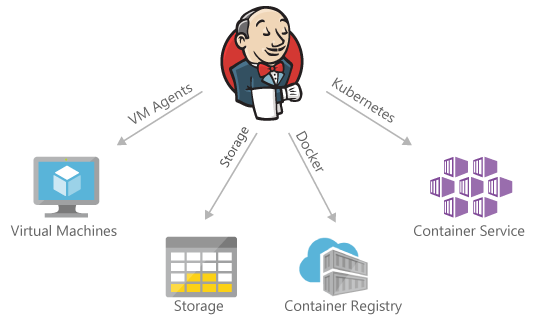
\includegraphics[width=0.48\textwidth]{./Images/Screenshot1.png}
  \end{center}
  \caption{Microsoft Azure Jenkins Angebot\cite{jenkins-azure}}\label{fig:Screenshot1}
\end{wrapfigure}

Direkt im Downloadbereich der Jenkins Seite wird ein Angebot von Microsoft Azure beworben. Dabei handelt es sich um eine bereits für den direkten Einsatz vorbereitete Ubuntu VM mit installiertem Jenkins und GIT. Man kann somit gegen eine monatliche Gebühr einen Jenkins Server weitestgehend sorgenfrei betreiben, da man sich nur um Jenkins selbst, nicht aber um die Infrastruktur kümmern muss. \cite{jenkins-azure}\\
In \autoref{fig:Screenshot1} ist das von Microsoft stammende Werbebild für Jenkins in Azure zu sehen. Daraus ist auch zu entnehmen, dass das Skalieren der Build Farm in Azure keine Hürde darstellt. Sowohl Build Agenten zum Bauen, Speicherplatz für das Ergebnis, wie auch Container inklusive Orchestrierung zum Testen sind in Azure möglich.
\section{Funktionsumfang \& Erweiterungsmöglichkeiten}
Jenkins selbst ist ohne Plugins sehr limitiert in seinen Funktionen. Jenkins verwaltet einzelne abgeschlossene Bereiche in sogenannten Projekten. In solchen Projekten kann dann unter Zuhilfenahme von Plugins ein Build aufgesetzt werden.\\
Es gibt ein Rechte-/Rollensystem, mit dem der Zugriff auf das System selbst, sowie auf einzelne Projekte festgelegt wird. Selbst ohne Erweiterungen kann man eine Master/Slave Beziehung zu anderen ausführenden Instanzen (sogenannten Agents) erstellen, mit deren Hilfe man die Last von Builds verteilen kann.\\
Das mächtigste Feature von Jenkins ist sein Plugin-System, für das es eine riesige Menge an bereits vorhandenen Plugins gibt, die zur Installation bereitstehen.
\subsection*{Erweiterungsmöglichkeiten}
Das bereits angesprochene Plugin-System von Jenkins erlaubt es, das System an sehr vielen Stellen zu erweitern. Dazu gibt es eine riesige Auswahl an bereits vorhandenen Erweiterungen, mit deren Hilfe die häufigsten Aufgaben bereits zu bewältigen sind. In \autoref{table:Jekins-Plugins} hat der Autor eine kleine Auswahl an vorhandenen Plugins zusammengestellt. Falls diese Auswahl nicht ausreicht, existieren in einer immensen Zahl von Paketen Extension Points für die man eigene Verbesserungen entwickeln kann, beispielsweise \cite{jenkins-extensionpoints} listet mehr als 180 Packages in denen Extension Points existieren.\\
In \autoref{sec:Gründe Continuous Integration einzusetzen} wurde als einer der Gründe für den Einsatz von CI der sogenannte Audit Trail erwähnt. Die Jenkins Plugin Bibliothek bietet bereits ein Plugin, das die Verantwortlichen bei dieser Aufgabe unterstützt:\\
Mit Hilfe des Audit Trail Plugins von Jenkins kann nachvollzogen werden, wer bestimmte Operationen ausgeführt hat, und zu welchem Zeitpunkt dies stattfand. Ein Beispiel für solch eine Aktion ist das Konfigurieren eines Jobs im Server. \cite{jenkins-audit-trail}\\
Dies unterstützt eine regelmäßig stattfindende Überprüfung durch beispielsweise die FDA enorm, da diese Information dann einfach nur noch extrahiert werden muss um sie dem Auditor verfügbar zu machen.
\begin{center}
  \begin{tabularx}{\textwidth}{lX}
    \toprule
    Kategorie & Plugins (Version, Stand: 14.08.2018) \\
    \midrule
    SCM &  TFSVC (5.139.2), GIT (3.9.1), Mercurial (2.4), CVS (2.14), Subversion (2.11.1) \\
		\addlinespace
    Buildtools & Ant (1.8), Maven (3.1.2), Gradle (1.29), MSBuild (1.29), PowerShell (1.3)\\
		\addlinespace
		Test & JUnit (1.24), NUnit (0.23), MSTest (0.23) \\
		\addlinespace
		Artefakte & Publish over SSH (1.19.1), Deploy to container (1.13), Publish over FTP (1.15), Artifact Deployer (1.2), Nexus Artifact Uploader (2.10)\\
		\addlinespace
		Werkzeuge & Mailer (1.21), Credentials (2.1.18), LDAP (1.20), Workspace Cleanup (0.34)\\
    \bottomrule
  \end{tabularx}
	\captionof{table}{Vorhandene Jenkins Plugins \cite{Jenkins-Plugins}}
	\label{table:Jekins-Plugins}
\end{center}
